\documentclass[11pt]{beamer}
%\usetheme{Boadilla}
\usepackage[utf8]{inputenc}
\usepackage[english]{babel}
\usepackage{amsmath}
\usepackage{amsfonts}
\usepackage{amssymb}
\usepackage{graphicx}
\usepackage{tikz}
\usefonttheme[onlymath]{serif}

\author{Alan Szepieniec}
%\title{}
\setbeamercovered{transparent} 
\setbeamertemplate{navigation symbols}{} 
%\logo{} 
%\institute{} 
%\date{} 
%\subject{} 
\begin{document}

%\begin{frame}
%\titlepage
%\end{frame}

%\begin{frame}
%\tableofcontents
%\end{frame}

\begin{frame}{}
\centering
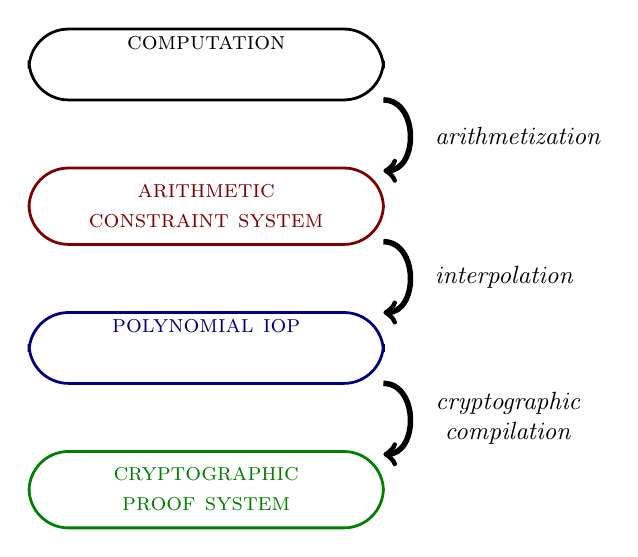
\begin{tikzpicture}[scale=0.9, every node/.style={scale=0.9}]
\node[draw, line width=1, rounded corners=0.5cm, minimum width=5cm, minimum height=1cm] (computation box) at (0,0) {};
\node[anchor=north] (computation label) at (computation box.north) {\textsc{computation}};

\node[draw, line width=1, rounded corners=0.5cm, minimum width=5cm, minimum height=1cm, color=red!50!black] (arithmetic constraint system box) at (0, -2) {\begin{tabular}{c}
\textsc{arithmetic} \\
\textsc{constraint system}
\end{tabular}};

\node[draw, line width=1, rounded corners=0.5cm, minimum width=5cm, minimum height=1cm, color=blue!50!black] (polynomial iop box) at (0, -4) {};
\node[anchor=north, color=blue!50!black] (polynomial iop label) at (polynomial iop box.north) {\textsc{polynomial iop}};

\node[draw, line width=1, rounded corners=0.5cm, minimum width=5cm, minimum height=1cm, color=green!50!black] (cryptographic proof system) at (0,-6) {\begin{tabular}{c}
\textsc{cryptographic} \\
\textsc{proof system}
\end{tabular}};

%\pause
%
%\node[] (bits) at (-4.5, 0) {$\{0,1\}^*, \wedge, \vee, \Leftrightarrow \!\!\neg$};
%
%\pause
%
%\node[] (field elements) at (-4.5, -2) {$\mathbb{F}^{\cdot \times \cdot}, \times, +, \circ, \cdot^\mathsf{T}$};
%
%\pause
%
%\node[] (polynomials) at (-4.5, -4) {$\mathbb{F}[X], z \xleftarrow{\S} \mathbb{F}, \langle \mathsf{P} \leftrightarrow \mathsf{V} \rangle$};
%
%\pause
%
%\node[] (crypto) at (-4.5, -6) {$\mathbb{F}, \mathsf{H}(\cdot), \mathsf{g}^x, \mathbf{A}s + e$};
%
%\pause

\draw[->, line width=2] (2.5, -0.5) .. controls (3, -0.5) and (3, -1.5) .. (2.5, -1.5) node[right, midway, xshift=0.2cm] {\textit{arithmetization}};

\draw[->, line width=2] (2.5, -2.5) .. controls (3, -2.5) and (3, -3.5) .. (2.5, -3.5) node[right, midway, xshift=0.2cm] {\textit{interpolation}};

\draw[->, line width=2] (2.5, -4.5) .. controls (3, -4.5) and (3, -5.5) .. (2.5, -5.5) node[right, midway] {\begin{tabular}{c}
\textit{cryptographic} \\
\textit{compilation}
\end{tabular}};
\end{tikzpicture}
\end{frame}

\begin{frame}
\centering
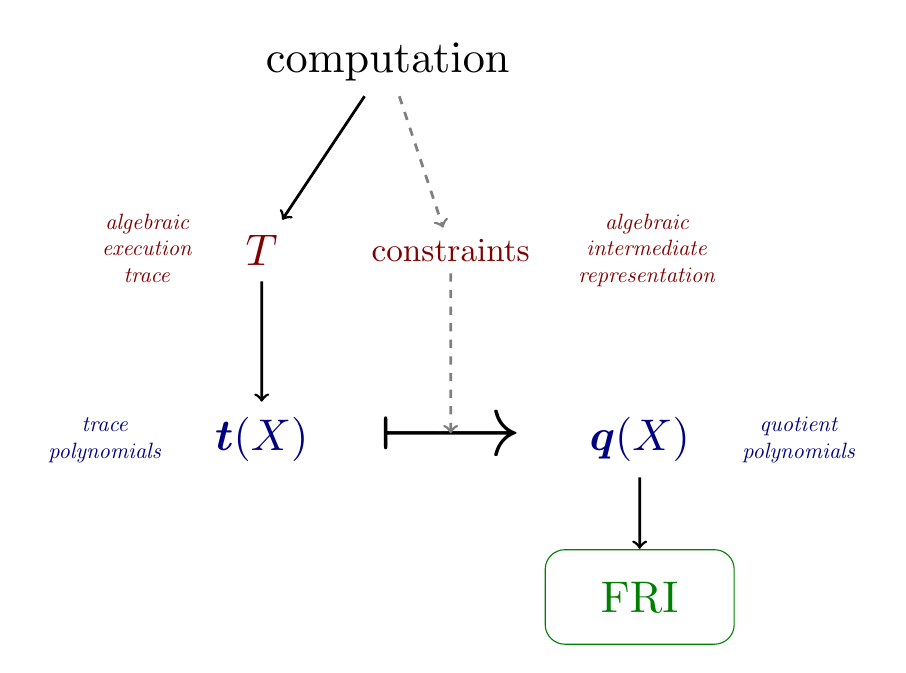
\begin{tikzpicture}[scale=0.8, every node/.style={scale=0.8}]
\node[scale=2, color=black] (computation) at (2, 6) {computation};

\node[scale=2, color=red!50!black] (trace) at (0, 3) {$T$};
\node[anchor=east, xshift=-0.25cm, color=red!50!black] (aet) at (trace.west) {\begin{tabular}{c}
\textit{algebraic} \\
\textit{execution} \\
\textit{trace}
\end{tabular}};

\node[scale=1.5, color=red!50!black] (constraints) at (3, 3) {constraints};
\node[anchor=west, xshift=0.25cm, color=red!50!black] (air) at (constraints.east) {\begin{tabular}{c}
\textit{algebraic} \\
\textit{intermediate} \\
\textit{representation}
\end{tabular}};

\draw[->, line width=1] (computation) -- (trace) {};
\draw[->, dashed, color=gray, line width=1] (computation) -- (constraints) {};

\node[scale=2, color=blue!50!black] (tx) at (0,0) {$\boldsymbol{t}(X)$};
\node[anchor=east, xshift=-0.25cm, color=blue!50!black] (trace polynomials) at (tx.west) {\begin{tabular}{c}
\textit{trace} \\
\textit{polynomials}
\end{tabular}};

\node[scale=4] (mapsto) at (3, 0) {$\longmapsto$};

\node[scale=2, color=blue!50!black] (qx) at (6, 0) {$\boldsymbol{q}(X)$};
\node[anchor=west, xshift=0.25cm, color=blue!50!black] (quotient polynomials) at (qx.east) {\begin{tabular}{c}
\textit{quotient} \\
\textit{polynomials}
\end{tabular}};

\draw[->, line width=1] (trace) -- (tx) {};
\draw[->, dashed, color=gray, line width=1] (constraints) -- (3,0.1) {};

\node[color=green!50!black, draw, rounded corners=0.25cm, scale=2, minimum width=1.5cm, minimum height=0.75cm] (fri) at (6, -2.5) {FRI};
\draw[->, line width=1] (qx) -- (fri) {};
\end{tikzpicture}
\end{frame}

\begin{frame}{}
\centering
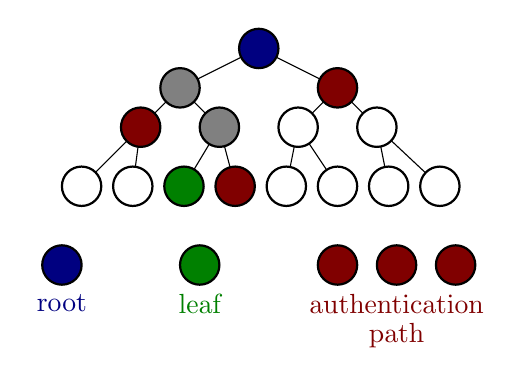
\begin{tikzpicture}[node distance=2.5cm,auto]
    \node [coordinate] (root) []{};
    \node [coordinate, yshift=-0.5cm, xshift=-1cm] (l) []{};
    \node [coordinate, yshift=-0.5cm, xshift=1cm] (r) []{};
    \node [coordinate, yshift=-0.5cm, xshift=-0.5cm] (ll) at (l) []{};
    \node [coordinate, yshift=-0.5cm, xshift=0.5cm] (lr) at (l) []{};
    \node [coordinate, yshift=-0.5cm, xshift=-0.5cm] (rl) at (r) []{};
    \node [coordinate, yshift=-0.5cm, xshift=0.5cm] (rr) at (r) []{};
    
    \node [coordinate, yshift=-0.75cm, xshift=-0.75cm] (lll) at (ll) []{};
    \node [coordinate, xshift=0.65cm] (llr) at (lll) []{};
    \node [coordinate, xshift=0.65cm] (lrl) at (llr) []{};
    \node [coordinate, xshift=0.65cm] (lrr) at (lrl) []{};
    \node [coordinate, xshift=0.65cm] (rll) at (lrr) []{};
    \node [coordinate, xshift=0.65cm] (rlr) at (rll) []{};
    \node [coordinate, xshift=0.65cm] (rrl) at (rlr) []{};
    \node [coordinate, xshift=0.65cm] (rrr) at (rrl) []{};
    
    \path[-] (root) edge (l);
    \path[-] (root) edge (r);
    \path[-] (l) edge (ll);
    \path[-] (l) edge (lr);
    \path[-] (r) edge (rl);
    \path[-] (r) edge (rr);
    \path[-] (ll) edge (lll);
    \path[-] (ll) edge (llr);
    \path[-] (lr) edge (lrl);
    \path[-] (lr) edge (lrr);
    \path[-] (rl) edge (rll);
    \path[-] (rl) edge (rlr);
    \path[-] (rr) edge (rrl);
    \path[-] (rr) edge (rrr);
    
    \draw [thick, fill=blue!50!black] (root) circle (0.25cm);
    \draw [thick, fill=gray] (l) circle (0.25cm);
    \draw [thick, fill=red!50!black] (r) circle (0.25cm);
    \draw [thick, fill=red!50!black] (ll) circle (0.25cm);
    \draw [thick, fill=gray] (lr) circle (0.25cm);
    \draw [thick, fill=white] (rl) circle (0.25cm);
    \draw [thick, fill=white] (rr) circle (0.25cm);
    \draw [thick, fill=white] (lll) circle(0.25cm);
    \draw [thick, fill=white] (llr) circle(0.25cm);
    \draw [thick, fill=green!50!black] (lrl) circle(0.25cm);
    \draw [thick, fill=red!50!black] (lrr) circle(0.25cm);
    \draw [thick, fill=white] (rll) circle(0.25cm);
    \draw [thick, fill=white] (rlr) circle(0.25cm);
    \draw [thick, fill=white] (rrl) circle(0.25cm);
    \draw [thick, fill=white] (rrr) circle(0.25cm);
    
    \node[coordinate] (root legend) at (-2.5, -2.75) {};
    \draw[thick, fill=blue!50!black] (root legend) circle (0.25cm);
    \node[anchor=north, yshift=-0.25cm, color=blue!50!black] (root label) at (root legend.south) {root};

    \node[coordinate] (leaf legend) at (-0.75, -2.75) {};
    \draw[thick, fill=green!50!black] (leaf legend) circle (0.25cm);
    \node[anchor=north, yshift=-0.25cm, color=green!50!black] (leaf label) at (leaf legend.south) {leaf};

	\node[coordinate] (authentication path legend 1) at (1, -2.75) {};
	\node[coordinate] (authentication path legend 2) at (1.75, -2.75) {};
	\node[coordinate] (authentication path legend 3) at (2.5, -2.75) {};
    \draw[thick, fill=red!50!black] (authentication path legend 1) circle (0.25cm);
    \draw[thick, fill=red!50!black] (authentication path legend 2) circle (0.25cm);
    \draw[thick, fill=red!50!black] (authentication path legend 3) circle (0.25cm);
    
    \node[anchor=north, yshift=-0.25cm, color=red!50!black] (authentication) at (authentication path legend 2.south) {authentication};
    \node[anchor=north, color=red!50!black, yshift=0.125cm] (path) at (authentication.south) {path};
	
    %\path[->] (start) edge node {} (e);
\end{tikzpicture}
\end{frame}

\begin{frame}{}
\centering
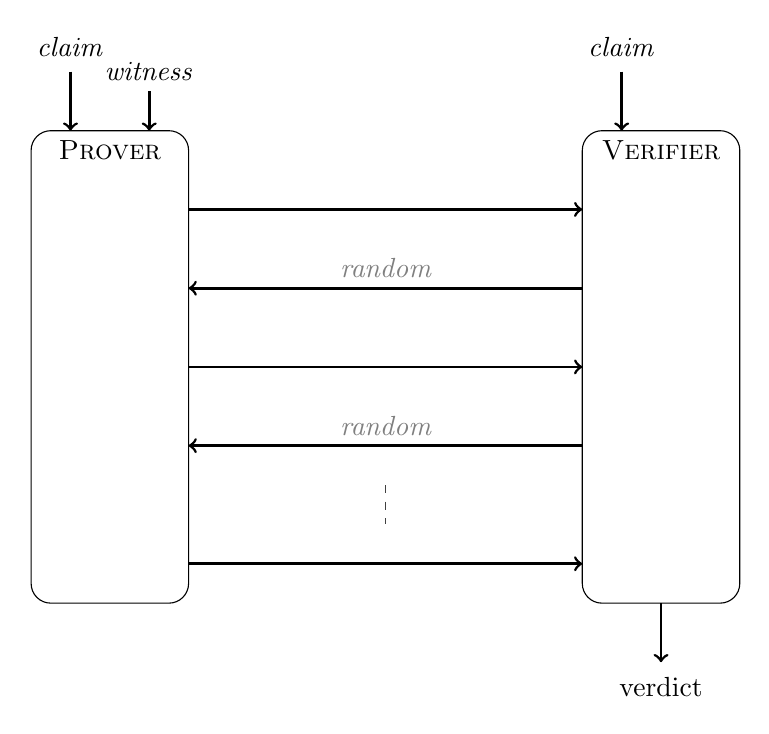
\begin{tikzpicture}
\draw[-, rounded corners=0.25cm] (-5, 0) -- (-6, 0) -- (-6, -6) -- (-4, -6) -- (-4, 0) -- (-5, 0) {};
\draw[-, rounded corners=0.25cm] (2, 0) -- (1, 0) -- (1, -6) -- (3, -6) -- (3, 0) -- (2, 0) {};

\node[anchor=north] (prover) at (-5, 0) {\textsc{Prover}};
\node[anchor=north] (verifier) at (2, 0) {\textsc{Verifier}};

\draw[->, line width=1] (-4, -1) -- (1, -1) {};
\draw[->, line width=1] (1, -2) -- (-4, -2) node[above, midway] {\textit{\textcolor{gray}{random}}};
\draw[->, line width=1] (-4, -3) -- (1, -3) {};
\draw[->, line width=1] (1, -4) -- (-4, -4) node[above, midway] {\textit{\textcolor{gray}{random}}};
\draw[dashed, color=gray!50!black] (-1.5, -4.5) -- (-1.5, -5) {};
\draw[->, line width=1] (-4, -5.5) -- (1, -5.5) {};

\draw[->, line width=1] (-5.5, 0.75) -- (-5.5, 0) node[above, near start, yshift=0.25cm] {\textit{claim}};
\draw[->, line width=1] (-4.5, 0.5) -- (-4.5, 0) node[above, near start, yshift=0.125cm] {\textit{witness}};

\draw[->, line width=1] (1.5, 0.75) -- (1.5, 0) node[above, near start, yshift=0.25cm] {\textit{claim}};

\draw[->, line width=1] (2, -6) -- (2, -6.75) node[below, near end, yshift=-0.25cm] {verdict};
\end{tikzpicture}
\end{frame}

\begin{frame}{}
\centering
\begin{tikzpicture}[overlay, yshift=2.5cm]
\draw[-, rounded corners=0.25cm] (-5, 0) -- (-6, 0) -- (-6, -6) -- (-4, -6) -- (-4, 0) -- (-5, 0) {};
\draw[-, rounded corners=0.25cm] (5, 0) -- (4, 0) -- (4, -6.5) -- (6, -6.5) -- (6, 0) -- (5, 0) {};
\draw[-, rounded corners=0.25cm, fill=black] (0,-0.5) -- (-0.5, -0.5) -- (-0.5, -6.5) -- (0.5, -6.5) -- (0.5, -0.5) -- (0, -0.5) {};

\node[anchor=north] (prover) at (-5, 0) {\textsc{Prover}};
\node[anchor=north] (proof stream) at (0, 0) {\textsc{Proof Stream}};
\node[anchor=north] (verifier) at (5, 0) {\textsc{Verifier}};

\draw[->, line width=1] (-4, -1) -- (-0.5, -1) {};
\draw[->, line width=1] (-0.5, -2) -- (-4, -2) node[above, midway] {\textit{pseudo\textcolor{gray}{random}}};
\draw[->, line width=1] (-4, -3) -- (-0.5, -3) {};
\draw[->, line width=1] (-0.5, -4) -- (-4, -4) node[above, midway] {\textit{pseudo\textcolor{gray}{random}}};
\draw[dashed, color=gray!50!black] (-2.5, -4.5) -- (-2.5, -5) {};
\draw[->, line width=1] (-4, -5.5) -- (-0.5, -5.5) {};

\draw[->, line width=1] (-5.5, 0.75) -- (-5.5, 0) node[above, near start, yshift=0.25cm] {\textit{claim}};
\draw[->, line width=1] (-4.5, 0.5) -- (-4.5, 0) node[above, near start, yshift=0.125cm] {\textit{witness}};

\draw[->, line width=1] (4.5, 0.75) -- (4.5, 0) node[above, near start, yshift=0.25cm] {\textit{claim}};

\draw[->, line width=1] (0.5, -6) -- (4, -6) node[above, midway] {\textit{serialized proof}};

\draw[->, line width=1] (5, -6.5) -- (5, -7.25) node[below, near end, yshift=-0.25cm] {verdict};
\end{tikzpicture}
\end{frame}

\begin{frame}{}
\centering
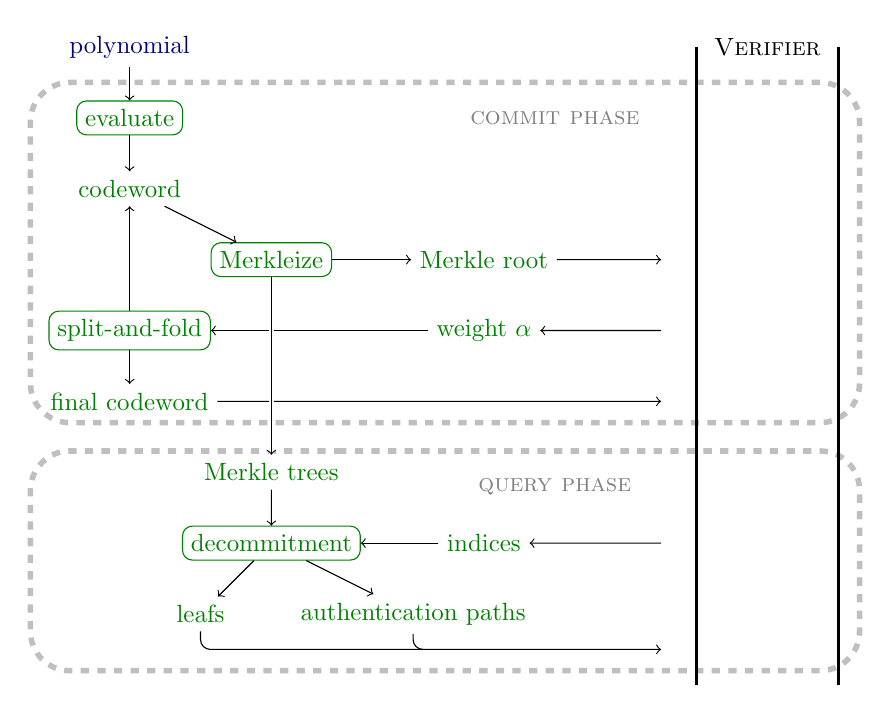
\begin{tikzpicture}[scale=0.9, every node/.style={scale=0.9}]

\draw[-, dashed, line width=2, color=gray!50!white, rounded corners=0.5cm] (3, -0.5) -- (-1.4, -0.5) -- (-1.4, -5.3) -- (10.3, -5.3) -- (10.3, -0.5) -- (3, -0.5) {};

\draw[-, dashed, line width=2, color=gray!50!white, rounded corners=0.5cm] (3, -5.7) -- (-1.4, -5.7) -- (-1.4, -8.8) -- (10.3, -8.8) -- (10.3, -5.7) -- (3, -5.7) {};

\node[color=gray] (commit phase) at (6, -1) {\textsc{commit phase}};
\node[color=gray] (commit phase) at (6, -6.2) {\textsc{query phase}};

\node[color=blue!50!black] (polynomial) at (0,0) {polynomial};
\node[draw, color=green!50!black, rounded corners=0.125cm] (evaluate) at (0, -1) {evaluate};
\draw[->] (polynomial) -- (evaluate) {};

\node[color=green!50!black] (codeword) at (0, -2) {codeword};
\draw[->] (evaluate) -- (codeword) {};

\node[draw, color=green!50!black, rounded corners=0.125cm] (merkleize) at (2, -3) {Merkleize};
\draw[->] (codeword) -- (merkleize) {};

\node[color=green!50!black] (merkle root) at (5, -3) {Merkle root};
\draw[->] (merkleize) -- (merkle root) {};

\draw[-, line width=1] (8, 0 ) -- (8, -9) {};
\draw[-, line width=1] (10, 0) -- (10, -9) {};
\node[] (verifier) at (9, 0) {\textsc{Verifier}};
\draw[->] (merkle root) -- (7.5, -3) {};

\node[color=green!50!black] (weight) at (5, -4) {weight $\alpha$};
\draw[->] (7.5, -4) -- (weight) {};

\node[draw, color=green!50!black, rounded corners=0.125cm] (split and fold) at (0, -4) {split-and-fold};
\draw[->] (weight) -- (split and fold) {};
\draw[->] (split and fold) -- (codeword) {};

\node[color=green!50!black] (final codeword) at (0, -5) {final codeword};
\draw[->] (split and fold) -- (final codeword) {};
\draw[->] (final codeword) -- (7.5, -5) {};

\node[color=green!50!black] (merkle trees) at (2, -6) {Merkle trees};
\draw[->, line width=2, color=white] (merkleize) -- (merkle trees) {};
\draw[->] (merkleize) -- (merkle trees) {};

\node[draw, color=green!50!black, rounded corners=0.125cm] (decommitment) at (2, -7) {decommitment};
\draw[->] (merkle trees) -- (decommitment) {};

\node[color=green!50!black] (indices) at (5, -7) {indices};
\draw[->] (7.5, -7) -- (indices) {};
\draw[->] (indices) -- (decommitment) {};

\node[color=green!50!black] (leafs) at (1, -8) {leafs};
\node[color=green!50!black] (paths) at (4, -8) {authentication paths};
\draw[->] (decommitment) -- (leafs) {};
\draw[->] (decommitment) -- (paths) {};

\draw[->, rounded corners=0.125cm] (leafs) -- (1, -8.5) -- (7.5, -8.5) {};
\draw[-, rounded corners=0.125cm] (paths) -- (4, -8.5) -- (4.125, -8.5) {};
\end{tikzpicture}
\end{frame}

\begin{frame}{}
\centering
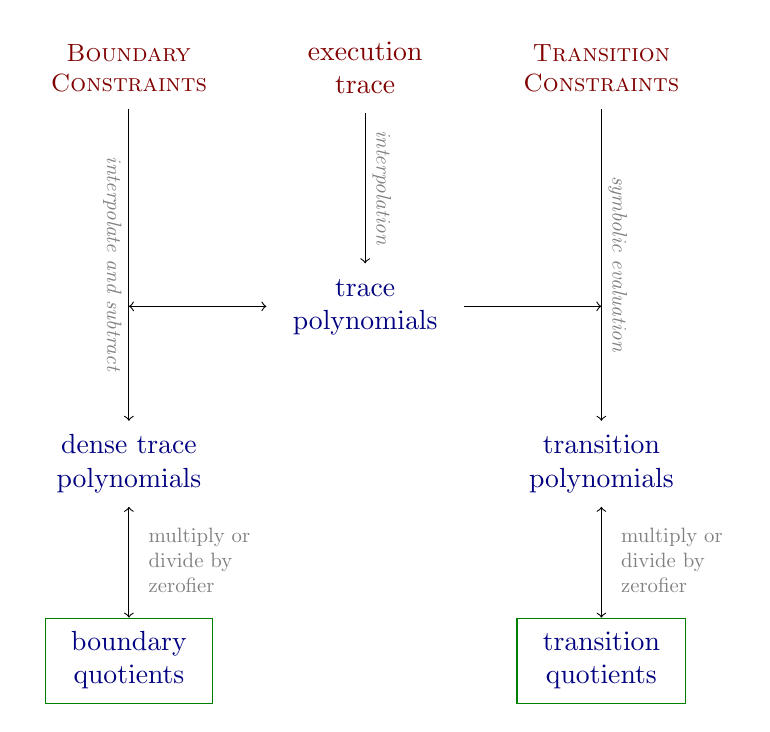
\begin{tikzpicture}
\node[color=red!50!black] (execution trace) at (0,0) {\begin{tabular}{c}
execution \\
trace
\end{tabular}};

\node[color=red!50!black, scale=0.9] (boundary constraints) at (-3, 0) {\begin{tabular}{c}
\textsc{Boundary} \\
\textsc{Constraints}
\end{tabular}};

\node[color=red!50!black, scale=0.9] (transition constraints) at (3, 0) {\begin{tabular}{c}
\textsc{Transition} \\
\textsc{Constraints}
\end{tabular}};

\node[color=blue!50!black] (trace polynomials) at (0, -3) {\begin{tabular}{c}
trace \\
polynomials
\end{tabular}};

\draw[->] (execution trace) -- (trace polynomials) node[above, midway, sloped, color=gray, scale=0.75] {\textit{interpolation}};

\node[color=blue!50!black] (dense trace polynomials) at (-3 ,-5) {\begin{tabular}{c}
dense trace \\
polynomials
\end{tabular}};
\node[color=blue!50!black] (transition polynomials) at (3 ,-5) {\begin{tabular}{c}
transition \\
polynomials
\end{tabular}};

\draw[->] (boundary constraints) -- (dense trace polynomials) node[below, midway, sloped, color=gray, scale=0.75] {\textit{interpolate and subtract}};
\draw[<->] (trace polynomials) -- (-3, -3) {};

\draw[->] (transition constraints) -- (transition polynomials) node[above, midway, sloped, color=gray, scale=0.75] {\textit{symbolic evaluation}};
\draw[->] (trace polynomials) -- (3, -3) {};

\node[draw, color=green!50!black] (boundary quotients) at (-3, -7.5) {\textcolor{blue!50!black}{\begin{tabular}{c}
boundary \\
quotients
\end{tabular}}};

\node[draw, color=green!50!black] (transition quotients) at (3, -7.5) {\textcolor{blue!50!black}{\begin{tabular}{c}
transition \\
quotients
\end{tabular}}};

\draw[<->] (dense trace polynomials) -- (boundary quotients) node[midway, right, color=gray, scale=0.75] {\begin{tabular}{l}
multiply or \\
divide by \\
zerofier
\end{tabular}};

\draw[<->] (transition polynomials) -- (transition quotients) node[midway, right, color=gray, scale=0.75] {\begin{tabular}{l}
multiply or \\
divide by \\
zerofier
\end{tabular}};
\end{tikzpicture}
\end{frame}

\begin{frame}{}
\centering
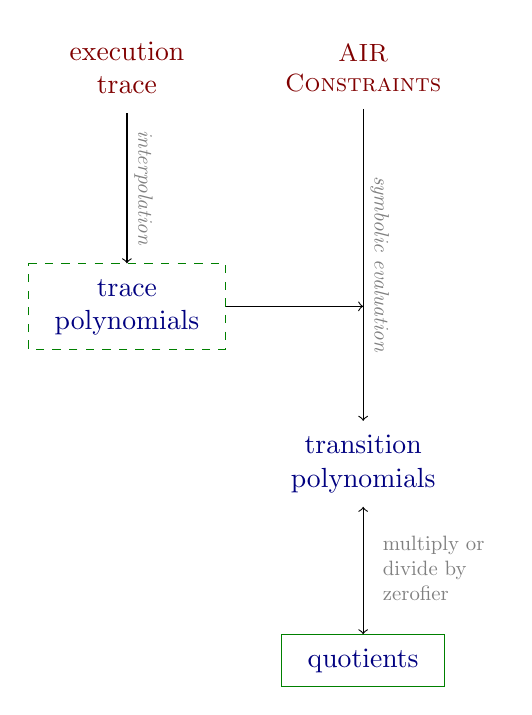
\begin{tikzpicture}
\node[color=red!50!black] (execution trace) at (0,0) {\begin{tabular}{c}
execution \\
trace
\end{tabular}};

\node[color=red!50!black, scale=0.9] (transition constraints) at (3, 0) {\begin{tabular}{c}
\textsc{AIR} \\
\textsc{Constraints}
\end{tabular}};

\node[] (trace polynomials) at (0, -3) {\begin{tabular}{c}
\textcolor{blue!50!black}{trace} \\
\textcolor{blue!50!black}{polynomials}
\end{tabular}};
\draw[dashed, color=green!50!black] (trace polynomials.north west) -- (trace polynomials.north east) -- (trace polynomials.south east) -- (trace polynomials.south west) -- (trace polynomials.north west) {};

\draw[->] (execution trace) -- (trace polynomials) node[above, midway, sloped, color=gray, scale=0.75] {\textit{interpolation}};

\node[color=blue!50!black] (transition polynomials) at (3 ,-5) {\begin{tabular}{c}
transition \\
polynomials
\end{tabular}};

\draw[->] (transition constraints) -- (transition polynomials) node[above, midway, sloped, color=gray, scale=0.75] {\textit{symbolic evaluation}};
\draw[->] (trace polynomials) -- (3, -3) {};

\node[draw, color=green!50!black] (transition quotients) at (3, -7.5) {\textcolor{blue!50!black}{\begin{tabular}{c}
quotients
\end{tabular}}};

\draw[<->] (transition polynomials) -- (transition quotients) node[midway, right, color=gray, scale=0.75] {\begin{tabular}{l}
multiply or \\
divide by \\
zerofier
\end{tabular}};
\end{tikzpicture}
\end{frame}

\begin{frame}{}
\centering
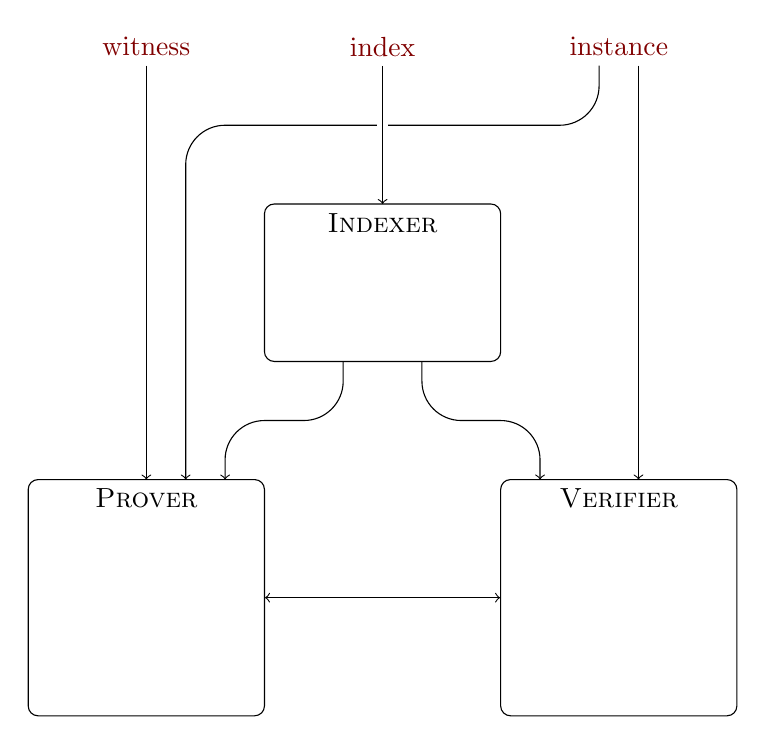
\begin{tikzpicture}
\node[color=red!50!black] (witness) at (-3, 0) {witness};
\node[color=red!50!black] (index) at (0, 0) {index};
\node[color=red!50!black] (instance) at (3, 0) {instance};

\node[minimum height=2cm, minimum width=3cm, draw, rounded corners=0.125cm] (indexer box) at (0, -3) {};
\node[anchor=north] (indexer label) at (indexer box.north) {\textsc{Indexer}};

\node[minimum height=3cm, minimum width=3cm, draw, rounded corners=0.125cm] (prover box) at (-3, -7) {};
\node[anchor=north] (prover label) at (prover box.north) {\textsc{Prover}};

\node[minimum height=3cm, minimum width=3cm, draw, rounded corners=0.125cm] (verifier box) at (3, -7) {};
\node[anchor=north] (verifier label) at (verifier box.north) {\textsc{Verifier}};

\draw[->, rounded corners=0.5cm] ([xshift=-0.25cm] instance.south) -- (2.75, -1) -- (-2.5, -1) -- (-2.5, -5.5) {};
\draw[-, color=white, line width=4] (index.south) -- (0, -1.5) {};
\draw[->] (index.south) -- (0, -2) {};

\draw[->] (witness.south) -- (-3, -5.5) {};

\draw[->] ([xshift=0.25cm] instance.south) -- (3.25, -5.5) {};

\draw[->, rounded corners=0.5cm] (-0.5, -4) -- (-0.5, -4.75) -- (-2, -4.75) -- (-2, -5.5) {};
\draw[->, rounded corners=0.5cm] (0.5, -4) -- (0.5, -4.75) -- (2, -4.75) -- (2, -5.5) {};

\draw[<->] (prover box) -- (verifier box) {};
\end{tikzpicture}
\end{frame}

\begin{frame}{}
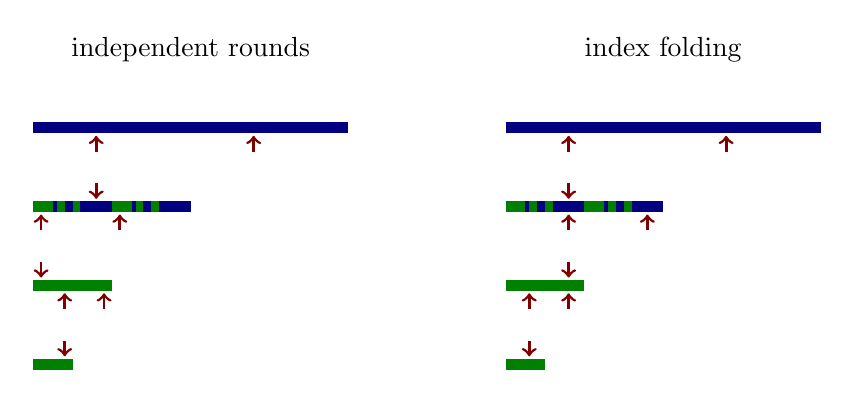
\begin{tikzpicture}
\begin{scope}[xshift=0]
\draw[-, line width=4, color=blue!50!black] (-4.5, 0) -- (-0.5, 0) {};
\draw[-, line width=4, color=blue!50!black] (-4.5, -1) -- (-2.5, -1) {};
\draw[-, line width=4, color=green!50!black] (-4.5, -1) -- (-4.25, -1) {};
\draw[-, line width=4, color=green!50!black] (-3.5, -1) -- (-3.25, -1) {};
\draw[-, line width=4, color=green!50!black] (-4.2, -1) -- (-4.1, -1) {};
\draw[-, line width=4, color=green!50!black] (-3.2, -1) -- (-3.1, -1) {};
\draw[-, line width=4, color=green!50!black] (-4, -1) -- (-3.9, -1) {};
\draw[-, line width=4, color=green!50!black] (-3, -1) -- (-2.9, -1) {};
\draw[-, line width=4, color=green!50!black] (-4.5, -2) -- (-3.5, -2) {};
\draw[-, line width=4, color=green!50!black] (-4.5, -3) -- (-4, -3) {};

\node[] (independent rounds) at (-2.5, 1) {independent rounds};

\draw[->, transform canvas={xshift=-2.7cm}, color=red!50!black, line width=1] (-1, -0.7) -- (-1, -0.9) {};
\draw[->, transform canvas={xshift=-2.7cm}, color=red!50!black, line width=1] (-1, -0.3) -- (-1, -0.1) {};
\draw[->, transform canvas={xshift=-0.7cm}, color=red!50!black, line width=1] (-1, -0.3) -- (-1, -0.1) {};

\draw[->, transform canvas={xshift=-3.4cm}, color=red!50!black, line width=1] (-1, -1.7) -- (-1, -1.9) {};
\draw[->, transform canvas={xshift=-3.4cm}, color=red!50!black, line width=1] (-1, -1.3) -- (-1, -1.1) {};
\draw[->, transform canvas={xshift=-2.4cm}, color=red!50!black, line width=1] (-1, -1.3) -- (-1, -1.1) {};

\draw[->, transform canvas={xshift=-3.1cm}, color=red!50!black, line width=1] (-1, -2.7) -- (-1, -2.9) {};
\draw[->, transform canvas={xshift=-3.1cm}, color=red!50!black, line width=1] (-1, -2.3) -- (-1, -2.1) {};
\draw[->, transform canvas={xshift=-2.6cm}, color=red!50!black, line width=1] (-1, -2.3) -- (-1, -2.1) {};

\end{scope}
\begin{scope}[xshift=6cm]
\draw[-, line width=4, color=blue!50!black] (-4.5, 0) -- (-0.5, 0) {};
\draw[-, line width=4, color=blue!50!black] (-4.5, -1) -- (-2.5, -1) {};
\draw[-, line width=4, color=green!50!black] (-4.5, -1) -- (-4.25, -1) {};
\draw[-, line width=4, color=green!50!black] (-3.5, -1) -- (-3.25, -1) {};
\draw[-, line width=4, color=green!50!black] (-4.2, -1) -- (-4.1, -1) {};
\draw[-, line width=4, color=green!50!black] (-3.2, -1) -- (-3.1, -1) {};
\draw[-, line width=4, color=green!50!black] (-4, -1) -- (-3.9, -1) {};
\draw[-, line width=4, color=green!50!black] (-3, -1) -- (-2.9, -1) {};
\draw[-, line width=4, color=green!50!black] (-4.5, -2) -- (-3.5, -2) {};
\draw[-, line width=4, color=green!50!black] (-4.5, -3) -- (-4, -3) {};

\node[] (index folding) at (-2.5, 1) {index folding};

\draw[->, transform canvas={xshift=-2.7cm}, color=red!50!black, line width=1] (-1, -0.7) -- (-1, -0.9) {};
\draw[->, transform canvas={xshift=-2.7cm}, color=red!50!black, line width=1] (-1, -0.3) -- (-1, -0.1) {};
\draw[->, transform canvas={xshift=-0.7cm}, color=red!50!black, line width=1] (-1, -0.3) -- (-1, -0.1) {};

\draw[->, transform canvas={xshift=-2.7cm}, color=red!50!black, line width=1] (-1, -1.7) -- (-1, -1.9) {};
\draw[->, transform canvas={xshift=-2.7cm}, color=red!50!black, line width=1] (-1, -1.3) -- (-1, -1.1) {};
\draw[->, transform canvas={xshift=-1.7cm}, color=red!50!black, line width=1] (-1, -1.3) -- (-1, -1.1) {};

\draw[->, transform canvas={xshift=-3.2cm}, color=red!50!black, line width=1] (-1, -2.7) -- (-1, -2.9) {};
\draw[->, transform canvas={xshift=-3.2cm}, color=red!50!black, line width=1] (-1, -2.3) -- (-1, -2.1) {};
\draw[->, transform canvas={xshift=-2.7cm}, color=red!50!black, line width=1] (-1, -2.3) -- (-1, -2.1) {};

\end{scope}

\end{tikzpicture}
\end{frame}

\end{document}